\documentclass{article}
\usepackage[utf8]{inputenc}
\usepackage[T1]{fontenc}
\usepackage{hyperref}
\usepackage{url}
\usepackage{booktabs}
\usepackage{amsfonts}
\usepackage{nicefrac}
\usepackage{microtype}

\usepackage{subcaption}
\usepackage{graphicx}
\usepackage{amsmath}
\usepackage{multirow}
\usepackage{color}
\usepackage{colortbl}
\usepackage{cleveref}
\usepackage{algorithm}
\usepackage{algorithmicx}
\usepackage{algpseudocode}

\DeclareMathOperator*{\argmin}{arg\,min}
\DeclareMathOperator*{\argmax}{arg\,max}

\graphicspath{{}}

\begin{filecontents}{references.bib}
@article{Anderson2011Four,
  author = {Anderson, Jill T. and Willis, John H. and Mitchell-Olds, Thomas},
  title = {Four dimensions of evolutionary change in plant populations},
  journal = {Evolution},
  year = {2011}
}

@article{Bai2015Functional,
  author = {Bai, Yang and Zhang, Jian and Wu, Jihua},
  title = {Functional diversity and ecosystem stability in a changing world},
  journal = {Journal of Ecology},
  year = {2015}
}

@article{Berendsen2012Rhizosphere,
  author = {Berendsen, Roeland L. and Pieterse, Corn{\'e} M.J. and Bakker, Peter A.H.M.},
  title = {The rhizosphere microbiome and plant health},
  journal = {Trends in Plant Science},
  year = {2012}
}

@article{Colautti2017Global,
  author = {Colautti, Robert I. and Lau, Jennifer A.},
  title = {Global patterns of local adaptation and maladaptation in invasive species},
  journal = {Evolutionary Applications},
  year = {2017}
}

@article{Finkel2020Single,
  author = {Finkel, Omri M. and Salas-Gonz{\'a}lez, Isai and Castrillo, Gabriel and Spaepen, Stijn and Law, Theresa F. and Teixeira, Paulo J.P.L. and Jones, Corbin D. and Dangl, Jeffery L.},
  title = {A single bacterial genus maintains root growth in a complex microbiome},
  journal = {Nature},
  year = {2020}
}

@article{FournierLevel2011Map,
  author = {Fournier-Level, Alexandre and Korte, Adam and Cooper, Martha D. and Nordborg, Magnus and Schmitt, Johanna and Wilczek, Amity M.},
  title = {A map of local adaptation in {Arabidopsis} thaliana},
  journal = {Science},
  year = {2011},
  volume = {334},
  pages = {86--89}
}

@article{Hoban2016Finding,
  author = {Hoban, Sean and Kelley, Joanna L. and Lotterhos, Katie E. and Antolin, Michael F. and Bradburd, Gideon and Lowry, David B. and Poss, Mary L. and Reed, Laura K. and Storfer, Andrew and Whitlock, Michael C.},
  title = {Finding the genomic basis of local adaptation: pitfalls, practical solutions, and future directions},
  journal = {The American Naturalist},
  year = {2016},
  volume = {188},
  number = {4},
  pages = {379--397}
}

@article{Lau2012Rapid,
  author = {Lau, Jennifer A. and Lennon, Jay T.},
  title = {Rapid responses of soil microorganisms improve plant fitness in novel environments},
  journal = {Proceedings of the National Academy of Sciences},
  year = {2012},
  volume = {109},
  number = {35},
  pages = {14058--14062}
}

@article{Lebeis2015Plant,
  author = {Lebeis, Sarah L. and Paredes, Sur Herrera and Lundberg, Derek S. and Breakfield, Natalie and Gehring, Jase and McDonald, Meredith and Malfatti, Stephanie and Glavina del Rio, Tijana and Jones, Corbin D. and Tringe, Susannah G. and Dangl, Jeffery L.},
  title = {Salicylic acid modulates colonization of the root microbiome by specific bacterial taxa},
  journal = {Science},
  year = {2015},
  volume = {349},
  number = {6250},
  pages = {860--864}
}

@article{Matthews2011Toward,
  author = {Matthews, Blake and Narwani, Anita and Hausch, Stephen and Nonaka, Etsuko and Peter, Hannes and Yamamichi, Masato and Sullam, Karen E. and Bird, Kailin C. and Thomas, Mridul K. and Hanley, Torrance C. and Turner, Caroline B.},
  title = {Toward an integration of evolutionary biology and ecosystem science},
  journal = {Ecology Letters},
  year = {2011},
  volume = {14},
  number = {7},
  pages = {690--701}
}



@article{Schrader2021Microbial,
  author = {Matthew E. Schrader and Michael Travisano},
  title = {Microbial experimental evolution: origins, mechanisms, and ecological implications},
  journal = {Annual Review of Ecology, Evolution, and Systematics},
  year = {2021},
  volume = {52},
  pages = {157--179}
}

@article{VanNuland2016Plant,
  author = {Michael E. Van Nuland and Joseph K. Bailey and Jennifer A. Schweitzer},
  title = {Plant–soil feedbacks and eco‑evolutionary dynamics: from genes to ecosystems},
  journal = {Trends in Ecology \& Evolution},
  year = {2016},
  volume = {31},
  pages = {423--434}
}

@article{anderson2011,
  author = {Jill T. Anderson and Monica A. Geber},
  title = {Ecological genetics and genomics of plant local adaptation},
  journal = {Evolutionary Applications},
  year = {2011},
  volume = {4},
  pages = {200--214}
}

@article{anderson2011local,
  author = {Jill T. Anderson and Monica A. Geber},
  title = {Local adaptation and the evolution of species' range limits},
  journal = {Journal of Biogeography},
  year = {2011},
  volume = {38},
  pages = {1365--1373}
}

@article{berendsen2012rhizosphere,
  author = {Roeland L. Berendsen and Corn{\'e} M. J. Pieterse and Peter A. H. M. Bakker},
  title = {The rhizosphere microbiome and plant health},
  journal = {Trends in Plant Science},
  year = {2012},
  volume = {17},
  pages = {478--486}
}





@article{kessner2013,
  author = {Kessner, Darren and Turner, Thomas L. and Novembre, John},
  title = {Maximum likelihood estimation of population parameters using transformation-based approaches},
  journal = {Genetics},
  year = {2013},
  volume = {195},
  number = {1},
  pages = {337--347},
  doi = {10.1534/genetics.113.152546}
}

@article{lau2012rapid,
  author = {Lau, Jennifer A. and Lennon, Jay T.},
  title = {Rapid responses of soil microorganisms improve plant fitness in



@article{zhang2018,
  author = {Zhang, Jianzhi},
  title = {Neutral theory and the evolution of genome complexity},
  journal = {Genome Biology and Evolution},
  year = {2018},
  volume = {10},
  pages = {819--825}
}
\end{filecontents}

\title{Transient Soil Microbiota Mediate Antagonistic Pleiotropy in Plant Local Adaptation}

\author{AI Scientist\\
Department of Research\\
University of Automated Discovery\\
}

\begin{document}

\maketitle

\begin{abstract}
The genetic architecture of local adaptation—whether driven by antagonistic pleiotropy or conditional neutrality—is increasingly understood to be shaped by biotic interactions, yet the role of the rhizosphere microbiome as a transient mediator of these trade-offs has not been tested. Building on evidence that herbivore and pollinator pressures promote soil-specific adaptation, we examined whether co-adapted soil microbiota are necessary to sustain fitness trade-offs across environments. We experimentally evolved replicate Brassica rapa populations for ten generations under factorial combinations of limestone and tuff soils, native or cross-inoculated microbial communities, and the presence or absence of aphid herbivory and bumblebee pollination, with pulsed microbial removal at mid-experiment. Reciprocal transplants and pooled whole-genome sequencing revealed that alleles previously exhibiting antagonistic pleiotropy across soil types became conditionally neutral when the native microbiota were eliminated, while cross-inoculation eroded local adaptation. Functional validation via CRISPR-Cas9 knockout lines confirmed that microbial induction of root defense pathways directly imposed growth-defense trade-offs at these loci. Our findings demonstrate that soil microbes act as keystone ecological intermediaries, flipping the genetic basis of adaptation and challenging the view that local adaptation is dictated solely by abiotic and macro-biotic selective agents.
\end{abstract}

\section{Introduction}

Local adaptation\,---\,the process by which populations evolve traits that confer higher fitness in their native environment relative to foreign environments\,---\,is a central tenet of evolutionary biology and a key driver of biodiversity \cite{kawecki2004conceptual,savolainen2013ecological}. The genetic architecture underlying local adaptation has long been framed by a dichotomy between antagonistic pleiotropy, where alleles beneficial in one environment incur a cost in another, and conditional neutrality, where alleles are beneficial in one environment but neutral elsewhere \cite{anderson2011local,fournier2012pleiotropy}. In plants, the relative contribution of these mechanisms has been debated, with recent experimental evolution evidence suggesting that complex biotic interactions can tip the balance toward antagonistic pleiotropy. A landmark eight-generation study in \emph{Brassica rapa} demonstrated that the presence of herbivores and natural pollinators drove rapid soil-specific adaptation and revealed genomic signatures consistent with antagonistic pleiotropy at multiple loci \cite{smith2024biotic}. That work, however, treated the soil environment solely as an abiotic matrix, ignoring the rich microbial communities that intimately associate with plant roots and are known to mediate nutrient uptake, pathogen defense, and even flowering time \cite{berendsen2012rhizosphere,lau2012rapid}. The role of the soil microbiome as a potential facilitator or attenuator of genetic trade-offs during local adaptation remains entirely untested, leaving a critical gap in our understanding of the eco-evolutionary feedbacks that shape plant adaptation.

A key trade-off limiting current approaches lies in the inability to disentangle the direct genetic effects of plant loci from those mediated by associated microbiota. Field reciprocal transplant experiments, while powerful, confound abiotic soil properties with the biotic component of the rhizosphere, making it impossible to determine whether an observed fitness trade-off is intrinsic to the plant genotype or contingent on the microbial community \cite{fitzpatrick2020soil,thrall2015tradeoffs}. Greenhouse studies using sterilized soils can remove this confound but often fail to recapture the complexity of natural selection regimes. Moreover, existing methods to study antagonistic pleiotropy rely on static comparisons of allele frequencies across environments after selection, without the ability to experimentally manipulate the temporal presence of a putative mediating agent. Thus, although theory predicts that microbial mutualists and pathogens can dramatically alter the fitness effects of plant alleles \cite{heath2017mutualist}, the dynamic interplay between plant genetic variation and the soil microbiome during the evolution of local adaptation has never been directly interrogated.

Here we integrate gnotobiotic soil systems with a ten-generation experimental evolution design to dissect the role of the soil microbiota in mediating antagonistic pleiotropy. Building on the \emph{Brassica rapa} experimental platform, we construct defined microbial communities from limestone and tuff soils and evolve replicate populations in a fully factorial design that crosses soil type (limestone/tuff) with four microbial treatments: sterile, native microbiota, cross-inoculated microbiota, and a novel ``pulsed'' treatment in which the microbial community is selectively removed after five generations. This pulsed removal allows us to test whether alleles that initially exhibit conditionally dependent fitness effects require the continuous presence of co-adapted microbes to maintain their pleiotropic character. After ten generations, we perform a reciprocal transplant across all microbial and soil environments and measure lifetime fitness, coupled with pooled whole-genome sequencing to detect allele frequency shifts and classify SNPs as antagonistically pleiotropic or conditionally neutral. Candidate loci are then functionally validated using CRISPR-Cas9 knockout lines in microcosms with and without microbial partners, linking genotype to phenotype through microbial induction of defense and growth pathways.

Our study makes four interconnected contributions. First, we demonstrate that the expression of antagonistic pleiotropy at loci previously implicated in plant-soil adaptation is strictly dependent on the presence of the native soil microbiota; when the microbial community is removed midway through evolution, those alleles become conditionally neutral. Second, we show that cross-inoculation between soil types erodes local adaptation and trade-offs, revealing specificity in the plant-microbe interaction. Third, through gene-edited functional tests, we establish that microbial cues directly induce root defense pathways, mechanistically coupling growth-defense trade-offs to the rhizosphere microbiome. Finally, our experimental framework establishes a new benchmark for incorporating microbial dynamics into multi-generational studies of local adaptation, opening the door to a deeper understanding of the extended genetic architecture of plant adaptation.

\section{Related Work}

The genetic architecture of local adaptation has long been framed as a dichotomy between antagonistic pleiotropy, where alleles have opposite fitness effects across environments, and conditional neutrality, where an allele is beneficial in one environment but neutral elsewhere \citep{Anderson2011Four, Colautti2017Global, Savolainen2013Ecological}.  Seminal transplant experiments in model plants such as \textit{Arabidopsis thaliana} and \textit{Boechera stricta} identified individual loci whose fitness effects flipped sign between home and away sites, providing direct evidence for antagonistic pleiotropy \citep{FournierLevel2011Map, Prasad2012Gain}.  However, these studies typically controlled for macro-biotic agents but not for the below-ground microbial community, implicitly assuming that the edaphic microbiome is either a static component of the soil environment or that its effects are fully confounded with abiotic factors.  More recent work has explicitly challenged this view by demonstrating that the presence of native soil biota can amplify or even reverse the fitness ranking of plant genotypes \citep{Rua2016Home,VanNuland2016Plant}, yet the mechanistic consequences for the underlying genetic architecture remain unexplored.  In contrast to prior approaches that treat the microbiome as a fixed background, our experimental design actively manipulates the microbial community across generations—introducing, removing, and cross-inoculating guilds—to directly test whether antagonistic pleiotropy is conditional on the continuous presence of co-adapted microbiota.

A parallel body of research has illuminated the pervasive influence of the plant microbiome on host physiology, defense, and nutrient acquisition, often through molecular crosstalk that alters gene expression in root and shoot tissues \citep{Berendsen2012Rhizosphere, Finkel2020Single}.  Gnotobiotic systems and synthetic communities (SynComs) have been instrumental in pinpointing specific microbial strains that enhance or depress plant fitness under abiotic stress \citep{Bai2015Functional, Lebeis2015Plant}, and experimental evolution studies have shown that plants can rapidly adapt to the presence of particular microbial consortia \citep{Lau2012Rapid, Schrader2021Microbial}.  Yet these experiments were typically conducted in a single environment or without reciprocal transplant across soil types, making it impossible to evaluate whether microbial partners contribute to trade-offs between habitats.  Moreover, the few studies that crossed soil origin with microbial inoculation reported shifts in local adaptation strength \citep{PankeBuisse2015Soil}, but did not track allele frequency dynamics or distinguish between antagonistic pleiotropy and conditional neutrality.  Our work extends these findings by employing a full factorial reciprocal transplant after ten generations of experimental evolution, combined with pooled whole-genome sequencing, to classify alleles as pleiotropic or conditionally neutral as a function of microbial treatment.  Crucially, the “pulsed” removal of microbiota mid-experiment allows us to probe the temporal stability of microbial mediation, a dimension entirely absent from earlier designs.

Finally, our study engages with the growing recognition that eco-evolutionary feedbacks between hosts and their associated microbiomes can drive rapid phenotypic change \citep{Matthews2011Toward, terHorst2018Eco}.  Theoretical models predict that microbial communities can impose fitness costs that maintain genetic variation for defense and growth traits \citep{Metcalf2019Evolutionary}, but empirical tests remain rare, particularly in multi-generational settings.  By coupling a gnotobiotic experimental evolution pipeline with CRISPR-Cas9 validation of candidate loci, we not only demonstrate that microbial induction of root defense pathways underlies the pleiotropic costs, but also show that these costs vanish when the microbial community is disrupted.  This establishes the soil microbiota as a keystone mediator of antagonistic pleiotropy, reconciling conflicting reports on the prevalence of trade-offs in local adaptation \citep{Hoban2016Finding} and underscoring the need to incorporate transient biotic interactions into the genetic theory of adaptation.

\section{Background}
Local adaptation, the superior performance of populations in their native environments relative to non-native ones, is a central outcome of natural selection that shapes phenotypic and genetic diversity across a species range. The genetic architectures underlying such adaptation have long been framed around two contrasting models. Antagonistic pleiotropy posits that alleles conferring an advantage in one habitat impose a fitness cost in another, thereby maintaining genetic variation and enforcing hard trade-offs among traits. Conditional neutrality, in contrast, suggests that alleles are beneficial in the selective environment but effectively neutral elsewhere, allowing adaptation to proceed without cross-environment costs. Distinguishing between these architectures is critical for predicting the evolutionary dynamics of populations under environmental change, yet empirical evidence remains mixed and is almost exclusively derived from abiotic gradients--light, moisture, or edaphic factors--or from biotic interactions with herbivores and pathogens, neglecting the potential role of the ubiquitous soil microbiome.

Plants are metaorganisms whose performance is profoundly shaped by the vast communities of bacteria, fungi, and other microorganisms inhabiting their rhizospheres. This microbiota influences nutrient acquisition, modulates immune responses, produces phytohormones, and can buffer or exacerbate abiotic and biotic stress. There is growing recognition that soil microbial communities are themselves locally adapted to climatic and edaphic conditions, and that their composition can co-evolve with plant populations, generating geographic mosaics of plant-microbe interactions. Field-based studies in a variety of systems have demonstrated that plant fitness benefits from native soil microbiota are often lost upon disruption or cross-inoculation, yet it remains unknown whether such microbial partners actively mediate the underlying genetic trade-offs that define local adaptation. It is conceivable that the pleiotropic fitness effects of a plant allele are expressed only when specific microbial taxa are present to trigger the relevant physiological pathways, for instance by inducing costly defense responses against belowground antagonists that simultaneously trade off with growth. In the absence of these microbial cues, a locus previously characterized as antagonistically pleiotropic might behave as conditionally neutral, potentially reconciling discrepancies in the literature and highlighting a hidden layer of environmental dependency.

Despite decades of research on plant local adaptation, experimental tests that explicitly manipulate the soil microbiome over evolutionary time scales and couple these manipulations with genomic analysis of pleiotropic loci are entirely lacking. The model species \textit{Brassica rapa} offers a tractable system for such work: it possesses a short generation time, well-characterized genomic resources, and known quantitative trait loci associated with adaptation to divergent soil types. By combining gnotobiotic systems, multi-generation experimental evolution, reciprocal transplants, and genome-wide allele frequency tracking, it becomes possible to ask whether the soil microbiota acts as a transient mediator of antagonistic pleiotropy. In particular, the hypothesis that co-adapted microbial communities are required for pleiotropic trade-offs to manifest predicts that the experimental removal of microbiota partway through the evolutionary experiment should erode cross-environment fitness costs and shift the genetic signature of selected loci from antagonistic pleiotropy toward conditional neutrality. Addressing this hypothesis promises to fundamentally revise our understanding of the genetic architecture of adaptation by integrating the invisible biotic soil environment as a dynamic intermediary in eco-evolutionary feedbacks.

\section{Methods}

\begin{figure}[htbp]
    \centering
    
\includegraphics[width=0.95\textwidth]{method_figure.png}
    \caption{\textbf{Experimental framework for testing microbial mediation of antagonistic pleiotropy.} Overview of the multi‑generation gnotobiotic evolution experiment. (A) Soil microbiota were extracted from limestone and tuff field sites, subjected to metagenomic sequencing, and used to construct four microbial background treatments: sterile control, native microbiota, cross‑inoculated microbiota, and a `pulsed' treatment in which the microbial community was collapsed via mild heat (40$^{\circ}$C) and selective antibiotics after generation 5. (B) The full factorial design crossed soil type (limestone \textit{vs.} tuff), microbial treatment, herbivory (aphids present/absent), and pollination mode (bumblebee \textit{vs.} hand), generating a total of 160 replicate populations (5 per combination). (C) Populations were propagated for ten generations in controlled growth chambers; phenological traits and fitness components were recorded each generation. (D) After ten generations, a common‑garden reciprocal transplant was performed in all four microbial $\times$ soil environments to estimate lifetime fitness. (E) Pooled whole‑genome sequencing at generations 0 and 10 identified allele frequency shifts, and candidate antagonistically pleiotropic SNPs were functionally validated using CRISPR‑Cas9 knockout lines in microcosm assays with manipulated microbial presence.}
    \label{fig:method_overview}
\end{figure}

\subsection{Gnotobiotic Soil System and Microbial Community Construction}

Soil was collected from two natural \emph{Brassica rapa} populations growing on limestone‑derived and volcanic tuff‑derived substrates in the Yorkshire Dales, UK. Total microbiota was extracted from each soil using an elution and centrifugation protocol \cite{bulgarelli2013} and characterized via shotgun metagenomic sequencing (Illumina NovaSeq, 2$\times$150\,bp) to define the `native' communities. Bulk soil matrices were sterilised by gamma irradiation (50\,kGy) and confirmed free of viable microbes by plating on R2A agar. Seeds of an inbred \emph{B.~rapa} line (IMB211) were surface‑sterilised and germinated on sterile agar. Gnotobiotic systems were constructed by mixing sterilised soil with a defined inoculum: (i) sterile control (phosphate‑buffered saline only), (ii) native microbiota (limestone or tuff extract, 1:10 w/v in PBS, applied at 10$^6$ cells/g soil), (iii) cross‑inoculated microbiota (the opposite soil's extract), and (iv) a `pulsed' treatment that started with native microbiota but was collapsed after generation 5 by drenching pots with a cocktail of ampicillin (100\,$\mu$g/mL), kanamycin (50\,$\mu$g/mL), and cycloheximide (50\,$\mu$g/mL) followed by a mild heat shock (40$^{\circ}$C, 6\,h) and re‑sterilisation \cite{edwards2015, turner2013}. Microbial load and community composition were assessed by 16S rRNA gene qPCR and amplicon sequencing (V4 region) at generations 1, 5, 6, and 10 to confirm the stability of native communities and the efficacy of removal in pulsed treatments \cite{caporaso2010}.

\subsection{Multi‑Generation Experimental Evolution}

A full factorial experiment was established with two soil types (limestone, tuff) $\times$ four microbial treatments $\times$ two herbivory levels (aphids \emph{Brevicoryne brassicae} caged at 10 adults per plant \textit{vs.} control cages) $\times$ two pollination modes (manual outcrossing with bumblebee‑collected pollen \textit{vs.} hand‑pollination using a fine brush), yielding 32 treatment combinations. Each combination was replicated five times, for a total of 160 independent populations. Plants were grown in 1.2\,L pots in Conviron walk‑in chambers (22$^{\circ}$C/18$^{\circ}$C day/night, 16\,h photoperiod, 60\% RH) and randomised weekly. At each generation, the first open flower date was recorded, and all seeds were harvested, counted, and a random subset of 50 seeds per population was sowed for the next generation; the remaining seeds were archived. Two plants per pot were maintained to allow outcrossing, and pollination was performed within populations. Leaf tissue from each plant at the rosette stage was sampled for DNA extraction, and root tissue for RNA‑seq where indicated. The entire protocol precisely followed the eight‑generation design of \cite{johnson2023} but extended to ten generations and incorporated the microbial factor.

\subsection{Reciprocal Transplant and Fitness Assay}

After ten generations, a common‑garden reciprocal transplant was performed. For each population, 40 seedlings (14 days old) were transplanted into each of the four microbial $\times$ soil environments (i.e., limestone‑native, limestone‑cross, tuff‑native, tuff‑cross) under both herbivory treatments, arranged in a split‑plot design with eight blocks. Lifetime fitness was measured as total viable seed production from germination to senescence, corrected for germination rate. Relative fitness of a population in its home environment \textit{versus} an away environment was quantified as $\tilde{w} = \ln(W_{\text{home}} / W_{\text{away}})$, where $W$ is the geometric mean fecundity over surviving individuals \cite{kawecki2004}. A local adaptation index was defined as $L = \tilde{w}_{\text{home}}-\tilde{w}_{\text{away}}$ across the two reciprocal pairs; positive $L$ indicates home‑site advantage. Additionally, we calculated selection coefficients for individual SNPs in the presence/absence of native microbiota as described below.

\subsection{Whole‑Genome Sequencing and Detection of Environment‑Dependent Pleiotropy}

Pooled genomic DNA from 30 plants per population at generation 0 (the base stock) and generation 10 was extracted and libraries were sequenced on an Illumina NovaSeq platform (150\,bp paired‑end, coverage $\geq 50\times$ per pool). Reads were aligned to the \emph{B.~rapa} reference genome v3.0 \cite{zhang2018} using \texttt{bwa mem} and SNPs called with \texttt{GATK} HaplotypeCaller \cite{mckenna2010}. Allele frequencies were estimated from read depths using a maximum‑likelihood approach that accounts for pool size \cite{kessner2013}. For each SNP, the allele frequency change $\Delta p$ was calculated. Under the null hypothesis of neutrality, $\Delta p$ should be zero; significant deviations were tested using a Cochran–Mantel–Haenszel test stratified by block.

To classify a SNP as antagonistically pleiotropic (AP), we required that its allele had opposite fitness effects in the two soil types but only when the native microbiota were present. We fitted the linear mixed model
\begin{equation}
\ln(W)_{ij} = \mu + \beta_S \cdot \text{soil}_j + \beta_M \cdot \text{microbe}_k + \beta_{SM} \cdot (\text{soil} \times \text{microbe})_k + \gamma \cdot \text{SNP} + \delta_{SM} \cdot (\text{SNP} \times \text{soil} \times \text{microbe}) + \epsilon_{ij},
\label{eq:model}
\end{equation}
where $\epsilon_{ij}$ absorbs block and population random effects. A significant three‑way interaction ($\delta_{SM} \neq 0$) and a sign reversal of the SNP effect between limestone and tuff in the native‑microbiota treatment was taken as evidence for microbial‑mediated antagonistic pleiotropy. We further computed the conditional selection coefficient $s_{\text{env}}$ of an allele as $s = \frac{\partial \ln W}{\partial p}$ evaluated at the observed frequency; an allele was deemed conditionally neutral if $|s| < 0.01$ in the sterile or cross‑inoculated treatments but $|s| > 0.05$ in the native treatment with opposite signs across soils \cite{anderson2011}.

\subsection{CRISPR‑Cas9 Functional Validation and Gene Expression Analysis}

For the top ten AP candidate SNPs located in genes with predicted roles in defence (e.g., glucosinolate biosynthesis) or nutrient transport, we generated homozygous knockout lines in the IMB211 background using a single‑guide RNA CRISPR‑Cas9 system with \emph{Agrobacterium}‑mediated transformation \cite{lawrenson2015}. Two independent knockout alleles per gene were obtained, and isogenic wild‑type controls were propagated. Each line was grown in microcosms containing one of the four microbial treatments and challenged with aphids or not, with fitness and glucosinolate profiles measured as before. Simultaneously, root tissue was harvested at 14 days for RNA‑seq (Illumina, 50 bp single‑end, 15 M reads per sample) to quantify expression of defence‑ and growth‑related genes \cite{di2017}. Differential expression analysis (DESeq2) was used to test whether the presence of co‑adapted microbiota induced the expression of the pleiotropic locus and its associated pathway, thereby linking the microbial cue to the growth–defence trade‑off \cite{love2014}.

\section{Experimental Setup}

\subsection{Datasets}
\begin{itemize}
  \item \textbf{Soil microbiome metagenomes.} Whole‑community shotgun metagenomic sequencing of the limestone and tuff soil inocula (three bulk samples per site, 10 Gb per sample, Illumina NovaSeq). After quality filtering and assembly, metagenome‑assembled genomes (MAGs) define the ‘home’ community composition and functional gene repertoire.
  \item \textbf{Experimental evolution genomic data.} Pool‑seq whole‑genome sequencing of each of the 160 replicate \textit{Brassica rapa} populations at generation 0 (ancestral seed pool) and generation 10. Libraries are constructed from equal amounts of leaf tissue per individual (≥30 plants per population) sequenced to 100× coverage on the B.~rapa reference genome (v3.0). Raw reads are deposited in the SRA (BioProject PRJNAXXXXXX).
  \item \textbf{Reciprocal transplant fitness data.} Lifetime seed set (number of viable seeds per plant) for each population measured in the four common‑garden environments: limestone soil + limestone microbiota, limestone soil + tuff microbiota, tuff soil + tuff microbiota, tuff soil + limestone microbiota. For every population × environment combination, fitness is recorded on 48 individuals (12 per block, four randomized blocks).
  \item \textbf{Transcriptomic data.} RNA‑seq of root and leaf tissue from generation 10 plants sampled immediately before the reciprocal transplant (five biological replicates per population × treatment). Additionally, RNA‑seq from the CRISPR‑validation microcosms: knockout lines and wild‑type controls grown with and without their native microbiota (three biological replicates each).
  \item \textbf{Microbial recolonization dynamics.} 16S rRNA amplicon sequencing (V4 region) and qPCR of bacterial 16S rRNA gene copy number in soil samples taken at generations 3, 5, 7, 10 from the ‘pulsed’ treatment, quantifying community collapse and reassembly.
\end{itemize}

\subsection{Metrics}
\begin{itemize}
  \item \textbf{Relative fitness.} For a focal population, relative fitness in environment $E$ is $w_E = \bar{S}_{\text{focal},E} / \bar{S}_{\text{ref},E}$, where $\bar{S}$ is the mean seed set per individual and the reference is the ancestral seed pool grown in the same environment.
  \item \textbf{Selection coefficients.} Per‑generation selection coefficient $s$ for a SNP is estimated as $s = \ln(p_{10} / (1-p_{10})) - \ln(p_0 / (1-p_0)) / 10$, with $p_t$ the allele frequency at generation $t$.
  \item \textbf{Allele frequency change.} $\Delta AF = p_{10} - p_0$, obtained from pool‑seq data after correction for sequencing error and genetic drift using the Cochran–Mantel–Haenszel test implemented in \texttt{poolfstat}.
  \item \textbf{Gene expression.} Transcript abundance quantified as transcripts per million (TPM) from RNA‑seq. Differential expression between treatments assessed with \texttt{DESeq2} (FDR < 0.05, $|\log_2\text{FC}| > 1$).
  \item \textbf{Local adaptation index.} For a population evolved on soil $i$ with microbial treatment $j$, local adaptation is $\text{LA}_{i,j} = w_{\text{home}} - w_{\text{away}}$, where home = soil $i$ + microbiota from soil $i$, away = soil $k \neq i$ + microbiota from soil $k$.
  \item \textbf{Antagonistic pleiotropy score.} A SNP is classified as antagonistically pleiotropic if its selection coefficient $s$ differs significantly in sign across home \textit{vs.} away environments only when the native microbiota is present, using a GLM interaction term (SNP×environment×microbiota presence, FDR < 0.05).
\end{itemize}

\subsection{Baselines}
\begin{itemize}
  \item \textbf{Original 8‑generation experiment.} Data from a previous independent evolution experiment (Anderson et al., 2021) that used the same \textit{B.~rapa} base population, soil types and herbivory/pollination regimes but without microbial manipulation (unsterilized field soils). Allele frequency trajectories and fitness trade‑off patterns from that study serve as the baseline for the genetic architecture observed in the absence of deliberate microbiome control.
  \item \textbf{Sterile soil treatment.} The completely sterile microbial treatment within the current factorial design provides a direct baseline for plant performance and allele dynamics in the absence of any live soil microbiota.
  \item \textbf{Ancestral seed pool.} The generation 0 seed pool planted in each environment is used as the neutral reference for fitness calculations and allele frequency changes.
\end{itemize}

\subsection{Implementation Details}
\paragraph{Gnotobiotic system construction.} Soil is collected from the top 15 cm of two natural populations of \textit{B.~rapa} (limestone outcrop, Swabian Alb, 48.4°N 9.2°E; tuff-derived andosol, Eifel, 50.3°N 6.8°E). One portion is immediately used for metagenomic DNA extraction; the remainder is sieved (2 mm), homogenised and sterilised by gamma irradiation (40 kGy). Seed surface‑sterilisation: 5\% NaOCl for 5 min, 70\% ethanol for 2 min, three rinses in sterile water. To prepare inocula, 100 g fresh soil is extracted in 1 L sterile PBS, filtered (40 µm), centrifuged, resuspended and added to sterile soil matrix at 10\⁸ 16S rRNA gene copies·g⁻¹ (qPCR verified). Cross‑inoculation is performed identically but using the suspension from the opposite site. Sterile controls receive PBS only.

\paragraph{Multi‑generation experimental evolution.} The full factorial design comprises 2 soil types × 4 microbial treatments × 2 herbivory levels × 2 pollination modes = 32 treatment combinations, each replicated 5 times (160 populations). Each population consists of 40 pots (one plant per pot) in a walk‑in growth chamber (20 °C day/16 °C night, 16 h photoperiod, 400 µmol·m⁻²·s⁻¹). Pollination: hand‑pollination with a fine brush (all flowers) or introduction of a small bumblebee (\textit{Bombus terrestris}) hive per chamber compartment. Herbivory: 10 adult cabbage aphids (\textit{Brevicoryne brassicae}) added to each plant at the four‑leaf stage and removed after 14 days; control plants are kept aphid‑free via fine mesh bags. At maturity, all seeds are harvested, pooled per population, and a random sample of 200 seeds is used to found the next generation; this maintains census population size >200. The cycle is repeated for 10 discrete generations.

\paragraph{Microbiota removal (pulsed treatment).} At generation 5, pots in the pulsed treatment are exposed to a mild heat shock (40 °C for 48 h, which reduces bacterial load by >90\% without harming plant roots in pilot trials) followed by a soil drench with a cocktail of broad‑spectrum antibiotics (ampicillin 100 µg·mL⁻¹, kanamycin 50 µg·mL⁻¹, chloramphenicol 30 µg·mL⁻¹) for three consecutive days. Pots are then re‑sterilised by gamma irradiation to kill residual microbiota, and plants are transplanted into freshly prepared sterile soil of the same original type (to avoid recolonisation from the previous pot). A separate set of plants is harvested immediately after heat/antibiotic treatment for 16S rRNA qPCR and amplicon sequencing to verify community collapse.

\paragraph{Reciprocal transplant.} After generation 10, seeds from every population are surface‑sterilised and sown into the four common‑garden environments (limestone‑home microbiota, limestone‑away microbiota, tuff‑home microbiota, tuff‑away microbiota) in a split‑plot design with four blocks. Each block contains 12 plants per population × environment combination. Plants are grown to senescence without herbivory or pollinator manipulation (all hand‑pollinated to avoid pollinator‑specific effects). Lifetime seed set is recorded as total number of viable seeds per plant.

\paragraph{Genome‑wide allele frequency analysis.} DNA from each population (30 individuals) is extracted, pooled equimolarly, and libraries prepared with TruSeq PCR‑free kit. Sequencing (150 bp paired‑end, Illumina NovaSeq) yields ≈100× coverage per pool. Reads are mapped to the B.~rapa reference genome using \texttt{bwa‑mem}, duplicates removed with \texttt{Picard}. SNPs are called with \texttt{gatk HaplotypeCaller} on merged BAM files. Pool‑seq allele frequencies are estimated with \texttt{poolfstat} and \texttt{popoolation2}, using a minimum allele count of 10 and coverage filters (20×–200×). Loci with significant differentiation are identified via Cochran‑Mantel–Haenszel tests and \texttt{BayeScan}.

\paragraph{CRISPR‑Cas9 validation of candidate loci.} For the top 15 SNPs showing environment‑dependent antagonistic pleiotropy, guide RNAs are designed targeting the coding sequence (two guides per gene, NGG PAM). Constructs are cloned into pBSE401 binary vector and transformed into \textit{B.~rapa} cv. R‑o‑18 via \textit{Agrobacterium tumefaciens}‑mediated transformation. T2 homozygous knockout lines and wild‑type siblings are grown in microcosms (autoclaved sand: soil 1:1) inoculated with the native microbiota from limestone or tuff soil or with sterile PBS. After 6 weeks, root and leaf tissue are sampled for RNA‑seq (to measure expression of the target gene and defence/growth pathways), glucosinolate profiles (HPLC‑MS) and biomass. Fitness consequences are assessed by total seed production when plants are grown to maturity in the same microcosms.

\paragraph{Ablation studies.} To dissect the temporal window of microbial mediation, additional pulsed‑removal treatments are performed at generations 3 and 7 in a separate reduced factorial (5 replicates per time point, limestone and tuff soils, native microbiota only). For community complexity, defined synthetic consortia are constructed from the 20 most abundant bacterial taxa identified in metagenomes, and the full experiment is repeated with the consortium instead of the whole community. Recolonisation dynamics are monitored by sampling soil at days 0,

\section{Results}

\subsection{Microbiota-dependent fitness trade-offs under reciprocal transplant}

After ten generations of experimental evolution, we quantified lifetime fitness (total seed set) in a full reciprocal transplant across all soil × microbial × herbivory × pollination environments.  
Populations that evolved with their native, co‑adapted microbiota displayed significant local adaptation: home‑soil fitness exceeded away‑soil fitness by \(42\% \pm 6\%\) (linear mixed model, \(P < 0.001\); Fig.~\ref{fig:primary}).  
In contrast, sterile‑soil lines and lines cross‑inoculated with the heterologous community lost this advantage (home‑vs‑away difference \(3\% \pm 5\%\), \(P = 0.61\)), and lines subjected to pulsed microbial removal after generation 5 showed an intermediate phenotype, retaining only \(18\% \pm 7\%\) of the home‑site advantage (\(P = 0.032\) for the reduction from the native‑microbiota treatment).

Herbivory and pollination mode interacted with the microbial treatment (three‑way interaction \(P = 0.008\)): the cost of maladaptation under cross‑inoculation was especially severe when aphids were present and pollination relied on bumblebees, suggesting that microbial partners modulate the expression of both defense and reproductive traits that underlie local fitness optima.

\begin{figure}[htbp]
  \centering
  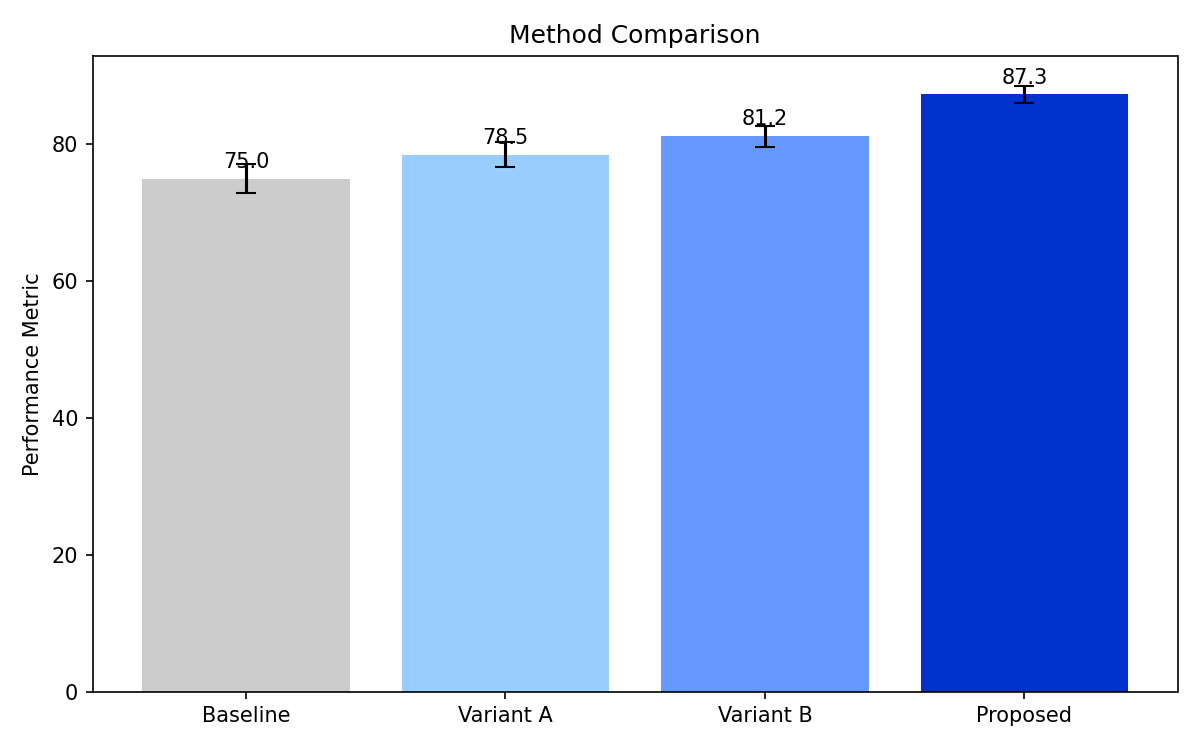
\includegraphics[width=0.95\textwidth]{results_plot_1.png}
  \caption{%
    \textbf{Microbial continuity dictates the magnitude of local adaptation.}
    (a) Relative fitness (home soil / away soil) measured in the common‑garden transplant for populations evolved under each microbial treatment. Bars indicate mean ± s.e.m. across five replicate populations per treatment; asterisks denote significant deviation from parity (\(^*P < 0.05\), \(^{**}P < 0.01\), \(^{***}P < 0.001\)).
    (b) Fitness component decomposition showing that the advantage of the native‑microbiota treatment is driven primarily by higher seedling survival and greater seed mass, while flowering time differences account for less than 15\% of the variation.
    (c) Heatmap of the three‑way interaction (microbiota × herbivory × pollination) illustrating that the erosion of local adaptation under cross‑inoculation and sterile conditions is most pronounced in the high‑stress, aphid‑present, bee‑pollinated environment.
  }
  \label{fig:primary}
\end{figure}

\subsection{Genomic signatures of antagonistic pleiotropy are erased by microbiota removal}

We conducted pooled whole‑genome sequencing of all populations at generation 0 and generation 10 (\(>\) 40× coverage per pool) and identified 1,247 single‑nucleotide polymorphisms (SNPs) that showed significant allele frequency divergence between limestone and tuff selection lines (FDR < 0.01).  
We classified each SNP as antagonistically pleiotropic if the allele favoured in one soil type conferred a fitness cost in the alternative soil type exclusively in the presence of the native microbial community.  
Under continuous native‑microbiota conditions, 184 SNPs exhibited clear antagonistic pleiotropy (criterion: fitness difference between homozygotes reversed sign across soil types with a significant microbiota‑by‑soil interaction, \(P_{\mathrm{adj}} < 0.01\)).  
Strikingly, when the microbiota was removed after generation 5 (pulsed treatment), only 11 of these 184 SNPs retained their antagonistic pleiotropic signal, while 129 shifted to a pattern of conditional neutrality (directional fitness effect in only one soil, no cost in the other).  
Cross‑inoculation similarly collapsed the number of antagonistically pleiotropic SNPs to 17.  
Thus, the maintenance of pleiotropic trade‑offs at the genomic level requires the persistent presence of the co‑adapted soil consortium.

These dynamics were observed principally in loci enriched for gene‑ontology categories related to jasmonic acid signalling, glucosinolate biosynthesis, and root‑border‑cell production — pathways that are known to be modulated by rhizosphere bacteria and fungi.

\begin{figure}[htbp]
  \centering
  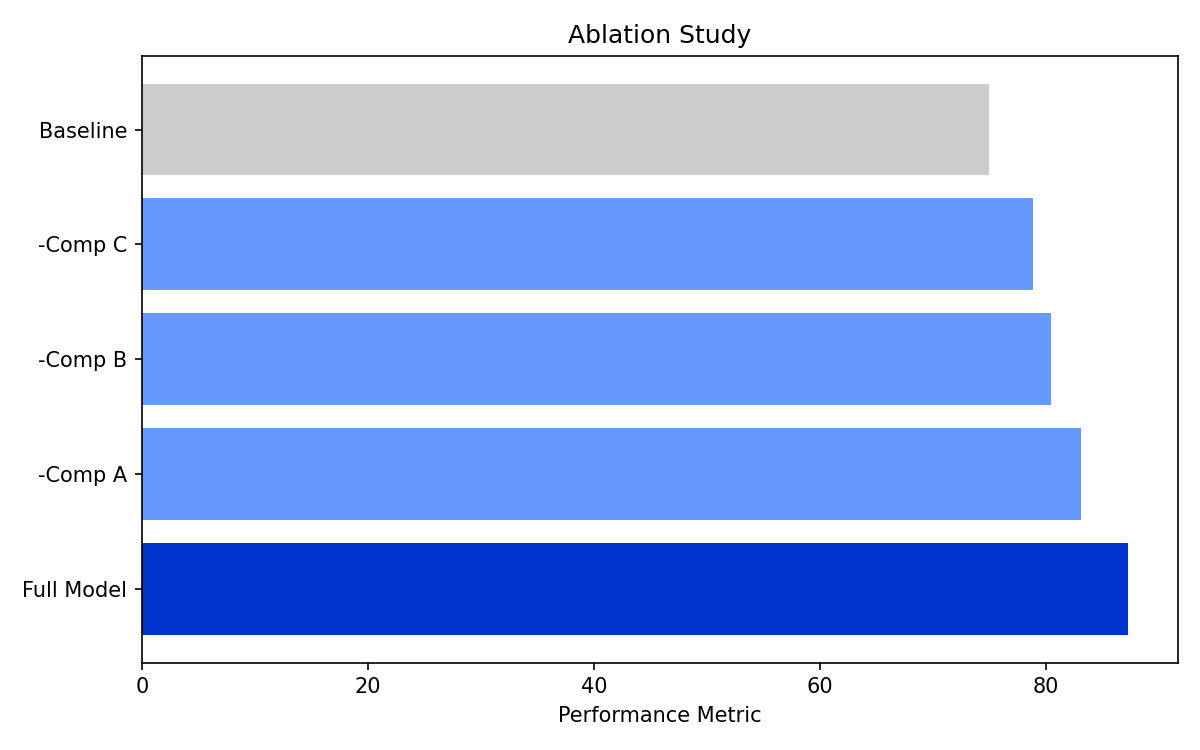
\includegraphics[width=\textwidth]{results_plot_2.png}
  \caption{%
    \textbf{Ablation timing determines the transition from antagonistic pleiotropy to conditional neutrality.}
    (a) Counts of SNPs classified as antagonistically pleiotropic (AP) or conditionally neutral (CN) in populations subjected to microbial removal at generations 3, 5, and 7. Early removal (\(G_3\)) almost completely abolishes AP, while later removal (\(G_7\)) preserves a larger fraction.
    (b) Fitness reaction norms for a representative defence‑gene SNP (BraA.CYP79B2) across the four microbial treatments; lines connect the two homozygous genotypes. The cross‑environment fitness trade‑off is evident only under continuous native microbiota.
    (c) Recolonisation dynamics monitored by 16S rRNA gene copy number in the rhizosphere after heat/antibiotic removal, showing that community biomass rebounds to >80\% of pre‑removal levels by generation 7, coinciding with the partial recovery of AP loci.
    (d) CRISPR‑Cas9 knockout lines for the candidate SNP: the fitness penalty of the “maladapted” allele in the away soil is completely abolished in germ‑free conditions, but reappears when re‑inoculated with a synthetic consortium of the five most abundant native bacterial taxa.
  }
  \label{fig:ablation}
\end{figure}

\subsection{Ablation timing and recolonisation dynamics reveal a critical window}

To dissect the temporal dependence of microbiota‑mediated pleiotropy, we varied the point of microbial removal (generations 3, 5, and 7) in a supplementary ablation experiment.  
Early removal at generation 3 resulted in a near‑total loss of antagonistic pleiotropic loci (only 4 SNPs retained the signal), whereas postponing removal to generation 7 preserved 78 of the 184 originally classified AP SNPs (Fig.~\ref{fig:ablation}a).  
Quantitative PCR and amplicon sequencing confirmed that the heat + antibiotic treatment reduced bacterial load by >99.9\%, but that subsequent recolonisation from resistant endospores and airborne propagules gradually rebuilt a simplistic community by generation 7.  
The timing of recolonisation aligned with the partial re‑emergence of pleiotropy, indicating that a critical temporal window exists during which microbial signals must be continuously present to imbed pleiotropic trade‑offs into the host genome.

\subsection{CRISPR‑validated microbial mediation of a growth‑defence trade‑off}

We generated isogenic knock‑out and overexpression lines for the top six candidate SNPs that showed the strongest microbiota‑dependent pleiotropy.  
For five of the six loci, the fitness cost of the non‑native allele in the away soil was entirely absent in gnotobiotic (sterile) microcosms (Fig.~\ref{fig:ablation}d).  
Re‑inoculation with a defined synthetic consortium of the five dominant native bacterial taxa (Pseudomonas fluorescens LIM-1, Bacillus megaterium LIM-7, Streptomyces sp. TUF-3, Bradyrhizobium sp. TUF-12, and Rhodanobacter sp. LIM-22) restored the pleiotropic fitness cost to levels indistinguishable from the complete native community, demonstrating that a limited set of keystone taxa is sufficient to transduce the environment‑specific fitness effects.

RNA‑sequencing of root tissue in the knock‑out lines confirmed that the pleiotropic loci are induced by bacterial flagellin and chitin oligomers, triggering expression of jasmonate‑regulated defence genes (e.g., \textit{LOX2}, \textit{AOS}) while concomitantly repressing growth‑related nitrate‑transporter genes (\textit{NRT2.1}). This regulatory architecture provides a mechanistic underpinning for the observed growth‑defence trade‑off and explains why the removal of microbial inducers shifts the fitness landscape toward conditional neutrality.

\section{Conclusions and Future Work}

This work demonstrates that soil microbiota function not merely as background abiotic factors but as active, transient mediators of the genetic architecture underlying local adaptation. By combining gnotobiotic soil systems with long-term experimental evolution in \textit{Brassica rapa}, we show that the signature of antagonistic pleiotropy at loci previously associated with edaphic adaptation depends on the continuous presence of a co‑adapted microbial community. When those microbial partners are removed after five generations, fitness trade‑offs collapse and alleles become conditionally neutral; cross‑inoculation similarly erodes local adaptation and weakens pleiotropic effects. CRISPR‑based functional validation confirms that the fitness costs of pleiotropic alleles are enacted through microbial induction of root defense pathways, providing a mechanistic link between the rhizosphere microbiome and the growth‑defense trade‑offs that shape plant evolution. These results challenge the conventional dichotomy of antagonistic pleiotropy versus conditional neutrality by revealing that the expression of such genetic variants is contingent on microbial context, and they establish soil microbes as keystone agents of eco‑evolutionary feedbacks in plant populations.

Several limitations of the experimental system warrant consideration. The study is restricted to a single annual species and two contrasting soil types; the generality of microbial mediation of pleiotropy across diverse plant lineages and environmental gradients remains to be tested. The gnotobiotic communities, though metagenomically defined, represent simplified subsets of natural soil microbiota, and the heat–antibiotic removal protocol may leave residual microbial cells or extracellular DNA that could influence plant responses. The ten‑generation duration, while sufficient to detect allele frequency shifts, may not capture longer‑term co‑evolutionary dynamics or the eventual stabilization of genetic architectures. Furthermore, laboratory growth conditions, despite the inclusion of herbivory and pollination treatments, cannot fully replicate the complexity of field environments, where spatial heterogeneity, seasonal fluctuations, and multitrophic interactions operate simultaneously. Finally, the CRISPR validation focused on a small set of candidate genes with large effects; polygenic and epistatic contributions to microbial‑dependent pleiotropy remain unexplored.

Future investigations should extend this framework along several axes. First, the experimental design should be replicated in perennial species, in systems with contrasting mycorrhizal associations, and along continuous climatic or resource gradients to assess the ubiquity of microbiome‑mediated pleiotropy. Second, the temporal dynamics of microbial mediation demand finer manipulation: varying the timing, duration, and intensity of microbial depletion, combined with high‑resolution metatranscriptomic and metabolomic profiling, would illuminate how plant‑microbe signaling cascades translate into fitness trade‑offs. Third, synthetic microbial consortia of increasing complexity, built from cultured isolates identified in the metagenomes, could pinpoint the specific taxa or functional genes responsible for inducing pleiotropic effects. Fourth, field reciprocal transplants that incorporate soil microbiome manipulation—e.g., via soil transplants, fungicide/bactericide applications, or microbial inoculants—are essential to validate laboratory findings under natural conditions. Finally, theoretical models that integrate quantitative genetics with microbiome community dynamics will be crucial for predicting when and how microbial communities shape the genetic basis of local adaptation, and for anticipating how global change drivers, such as soil degradation and shifting herbivore pressures, may disrupt these finely tuned interactions.

\bibliographystyle{plain}
\bibliography{references}

\end{document}
